\documentclass[letterpaper]{article}
\usepackage{hyperref}
\usepackage{multicol}
\usepackage{titlepic}
\usepackage{graphicx}
\usepackage[letterpaper, margin=1in]{geometry}

\setcounter{tocdepth}{2}

\title{18OC}
\author{Christopher Giroir}
\titlepic{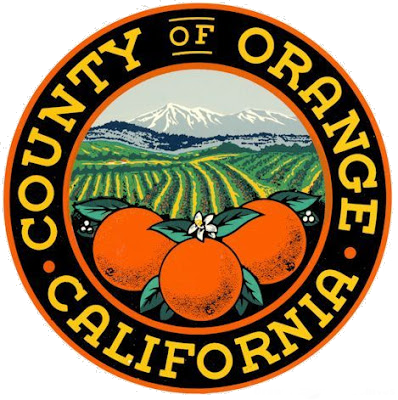
\includegraphics[width=\textwidth]{OC.png}}

\begin{document}

\maketitle

\newpage
\tableofcontents
\newpage

\begin{multicols}{2}
    \section*{Cheat Sheet}
    \begin{tabular}{l|l|l}
      \hline
      \textbf{Players} & \textbf{Cert Limit} & \textbf{Starting Capital} \\
      \hline
      \hline
      3 & 16 & \$400 \\
      4 & 13 & \$300 \\
      \hline
    \end{tabular}
    \subsection*{Stock Round}
    \begin{itemize}
    \item Sell then Buy
    \item Never more than 50\% in the pool
    \item Can not sell shares of companies which haven't completed an operating round
    \item Companies float at 2 shares sold, partial cap.
    \end{itemize}
    \subsection*{Operating Round}

    \begin{itemize}
    \item All player owned companies must own a train
    \item Privates may be bought in from half to double face value
    \end{itemize}

    \subsubsection*{Turn Sequence}
    \begin{enumerate}
    \item Lay one tile or upgrade
    \item Place a station token
    \item Run trains
    \item Pay out or withhold
    \item Buy trains
    \item Issue or Redeem shares
    \end{enumerate}

    \subsection*{Companies}

    \subsubsection*{Major Companies}
    \begin{enumerate}
    \item The California Southern Railroad (CSR), Southern California Railway (SCR)
    and the Santa Ana \& Newport Railway all function as standard 10 share
    companies
    \item The CSR opens as part of the initial auction
    \item The SCR and SNR along with the DRR open in a random order
    \item When all of these companies close, they get added to the queue of companies to open
    \item Can be restarted anywhere, no longer have a reserved home (DRR excepted)
    \end{enumerate}

    \subsubsection*{Pacific Electric}
    \begin{itemize}
    \item Never player owned
    \item Operates the round after Seal Beach is connected to Huntington Beach
    \item Starts at a share price of \$100
    \item Uses currently available train from the bank pool and always pays out
    \end{itemize}
    \subsubsection*{Disneyland Railroad}
    \begin{itemize}
    \item Home token permanently on the board in Anaheim, always blocks
    \end{itemize}
\end{multicols}
\end{document}
